\documentclass[conference]{IEEEtran}
\usepackage[T1]{fontenc}
\usepackage{graphicx}
\usepackage{booktabs}
\usepackage{amsmath}
\usepackage{url}
\usepackage{cite}
\usepackage{multirow}

\begin{document}

\title{Trust-Aware and Resource-Efficient Satellite Health Monitoring on ESA-ADB: A Pre-Registered Evaluation of Adaptive Computation, Sensor Reliability and Response Planning}

\author{\IEEEauthorblockN{Author One, Author Two, Author Three}
\IEEEauthorblockA{Department of Computer Science and Engineering\\
Institution Name, City, Country\\
\{author1, author2, author3\}@institution.edu}}

\maketitle

\begin{abstract}
Forecasting-based detectors such as Telemanom are a strong baseline for spacecraft telemetry monitoring, but they run a neural network on every reading, cannot tell a broken sensor from a real spacecraft problem, and miss most rare nominal events. We reproduce Telemanom-ESA on Mission~1 of the ESA Anomaly Detection Benchmark (ESA-ADB) and reach a corrected event-wise F0.5 of 0.801 against the published 0.776. On top of it we test six additions under a protocol fixed before any test-set run: a cheap screening tier that runs the LSTM only on demand (C1), a peer-consistency sensor-reliability layer (C2), dependency-graph incident correlation (C3), cost-aware response replay (C4), a calibrated error floor, and a telecommand-gated rare-event path. Every method is tuned on a labelled development period and run once on the 2007--2013 test set, with paired monthly-block bootstrap intervals over five seeds. C1 matches the baseline exactly while running the LSTM on 6.4\% of the data, a 20.3$\times$ end-to-end speed-up. On data with injected sensor faults, C2 raises F0.5 from 0.341 to 0.628 (95\% CI $[+0.22, +0.36]$) and does no harm on clean data. The learned graph and the learned response policy both lose to simpler alternatives, and the telecommand gates more than double rare-event detections without a confirmed overall gain. We report all results, including the negative ones.
\end{abstract}

\begin{IEEEkeywords}
anomaly detection, satellite telemetry, ESA-ADB, LSTM, adaptive computation, sensor faults, pre-registration
\end{IEEEkeywords}

\section{Introduction}
Spacecraft operators watch thousands of telemetry channels for behaviour that departs from normal. Forecasting detectors predict each channel from its recent past and raise an alarm when the forecast error becomes unusually large. Telemanom~\cite{hundman2018telemanom} established this design with an LSTM forecaster and nonparametric dynamic thresholding. The ESA Anomaly Detection Benchmark (ESA-ADB)~\cite{kotowski2024esaadb} later evaluated it on real ESA missions with operator-annotated events and a corrected event-wise F0.5 metric that penalises false alarms.

Three practical gaps remain. First, the network runs on every reading of every channel, even though most telemetry is plainly nominal. Second, every channel is treated as trustworthy, so a stuck or drifting sensor raises the same alarm as a real fault. Third, the baseline misses most rare nominal events, such as commanded operations, because their forecast errors are just below its pruning floor.

This paper reports a complete evaluation of additions aimed at these gaps. Our contributions are:
\begin{itemize}
\item A verified PyTorch reproduction of Telemanom-ESA on ESA-ADB Mission~1, scored with the official metric code, over five training seeds and two training lengths.
\item \textbf{C1, adaptive computation:} a cheap screening tier that sends only flagged bursts of telemetry to the LSTM. It is confirmed non-inferior, with a 20.3$\times$ speed-up.
\item \textbf{C2, sensor reliability:} a peer-consistency classifier that separates sensor faults from system events. It is confirmed on injected faults.
\item \textbf{C3--C4 and two further hypotheses:} incident correlation, cost-aware response, a calibrated floor and a telecommand-gated rare-event path. None beats its simpler comparison under the protocol. We report them with the same detail as the confirmed results.
\item \textbf{C5:} an ablation of the combined pipeline that identifies which parts carry the gains.
\end{itemize}
All designs, tuning grids and decision rules were committed to a dated protocol before their test runs. Each test was run once and logged.

\section{Related Work}
Telemanom~\cite{hundman2018telemanom} forecasts telemetry with an LSTM and flags anomalies with a nonparametric dynamic threshold on smoothed errors. ESA-ADB~\cite{kotowski2024esaadb} provides three ESA missions with labelled anomalies and rare events, telecommands, a time-aware evaluation pipeline, and published results for Telemanom-ESA and its ``Pruned'' variant.

Zeng et al.~\cite{zeng2022causal} combine a transfer-entropy causal network between telemetry parameters with a feature-attention LSTM and a dynamic $k$-sigma threshold. Their causal network motivates our dependency-graph grouping (C3). Xu et al.~\cite{xu2023taae} propose a temporal-attention LSTM autoencoder with a Mahalanobis anomaly score, an adaptive threshold and per-parameter attribution, which relates to our sensor-level attribution (C2). Zhang and Hu~\cite{zhang2025fouriergat} model cross-channel and temporal structure with a Fourier graph attention network. Mathur et al.~\cite{mathur2026adeptrs} study the robustness of telemetry detectors under evasion and poisoning attacks, a different aspect of trustworthy monitoring.

These works improve the forecaster or the anomaly score. Our seed study (Section~\ref{sec:repro}) shows that on ESA-ADB the decision layer after the forecaster decides which events are caught, so we target that layer, its compute cost and its trust in the sensors.

\section{Data, Baseline and Protocol}
\subsection{Data}
We use ESA-ADB Mission~1, channels 41--46 (the benchmark's lightweight subset, all in subsystem~5), on the official 30-second zero-order-hold grid. The training periods are 2000-01 to 2001-09 (21 months, 1,840,321 rows) and 2000-01 to 2006-12 (84 months). The test period, 2007--2013, contains 65 labelled events: 29 anomalies and 36 rare nominal events. For C3 we also prepare all 76 Mission~1 channels. For the rare-event path we use the mission's 698 telecommands, each with an ESA-assigned priority.

\subsection{Baseline and reproduction}\label{sec:repro}
Telemanom-ESA is a two-layer LSTM (80 units, dropout 0.3) that reads 250 samples of all six channels and predicts the next 10. The original \texttt{errors.py} turns the smoothed errors into alarms. The Pruned variant ignores errors below a floor of 0.007. Because the official TensorFlow~2.5.1 container does not support our GPU (RTX~5060), we ported the model to PyTorch. We kept the Keras initialisation, optimiser settings, epoch length and early-stopping rule, and we used the original thresholding code and the official \texttt{ESAScores} metric unchanged.

Table~\ref{tab:repro} compares our results with the paper. Pruned reaches F0.5 0.801 on every one of five seeds at 21 months. The five networks flag different samples but catch the same 29 events, so the error floor, not the forecaster, decides the result. At 84 months Pruned scores 0.784 against the published 0.786. The unpruned variant falls short of the paper: it has lower precision at the same recall. We attribute this to numerical differences between the two frameworks.

\begin{table}[t]
\caption{Reproduction: corrected event-wise F0.5, mean of 5 seeds (range)}\label{tab:repro}
\centering
\begin{tabular}{llcc}
\toprule
Training & Variant & Ours & Paper~\cite{kotowski2024esaadb} \\
\midrule
21 months & Telemanom-ESA & 0.105 (0.084--0.117) & 0.122 \\
          & Pruned        & \textbf{0.801} (all 0.801) & 0.776 \\
84 months & Telemanom-ESA & 0.106 (0.087--0.141) & 0.178 \\
          & Pruned        & \textbf{0.784} (0.773--0.791) & 0.786 \\
\bottomrule
\end{tabular}
\end{table}

\subsection{Evaluation protocol}
The 21-month models never see 2001-10 to 2006-12. This labelled period (33 events) serves as a development set for all tuning, and the test period is used once per hypothesis. The primary metric is corrected event-wise F0.5 over anomalies and rare events, averaged over seeds 42, 1, 2, 3 and 4.

For intervals we split the test period into 85 calendar months and decompose the metric into per-month counts: detected and missed events, false-alarm events and false-alarm time. We then resample months with replacement~\cite{kunsch1989block,efron1993bootstrap}, 5,000 times, scoring both systems on the same resample. The decomposition reproduces the official scores exactly.
\begin{itemize}
\item \emph{Improvement claim:} the whole 95\% interval of the difference lies above zero.
\item \emph{Non-inferiority claim:} for compute-saving methods, the lower bound must lie above $-0.02$.
\end{itemize}
The protocol names Holm's correction~\cite{holm1979} across hypotheses. We report unadjusted intervals. Both confirmed results lie far from their decision boundaries.

\section{Methods}
\begin{figure*}[t]
\centering
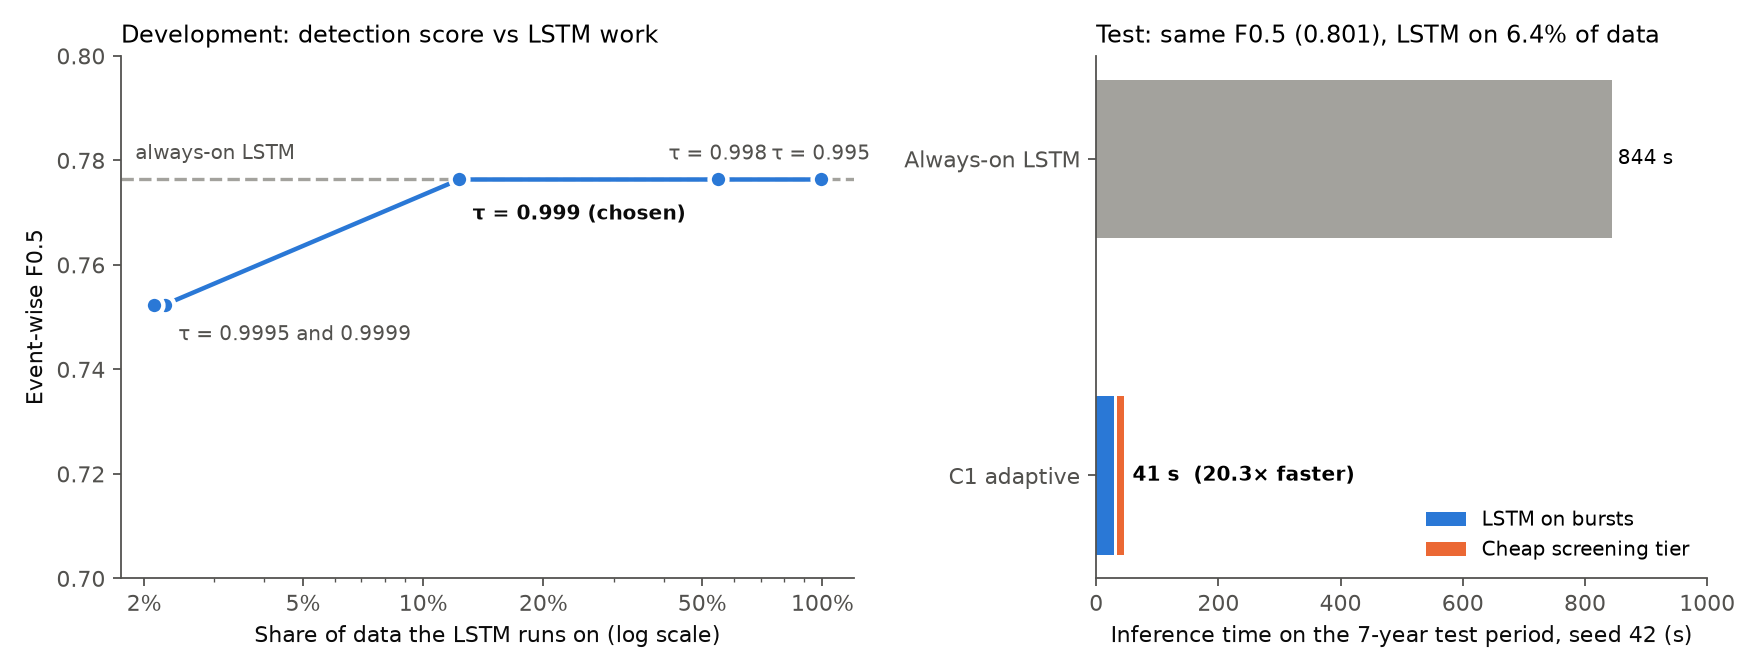
\includegraphics[width=0.88\textwidth]{figures/7_c1_adaptive_computation.png}
\caption{C1. Left: development F0.5 against the share of data the LSTM runs on, for screening thresholds $\tau$ from 0.995 to 0.9999. Right: measured test-period inference time.}
\label{fig:c1}
\end{figure*}

\begin{figure*}[t]
\centering
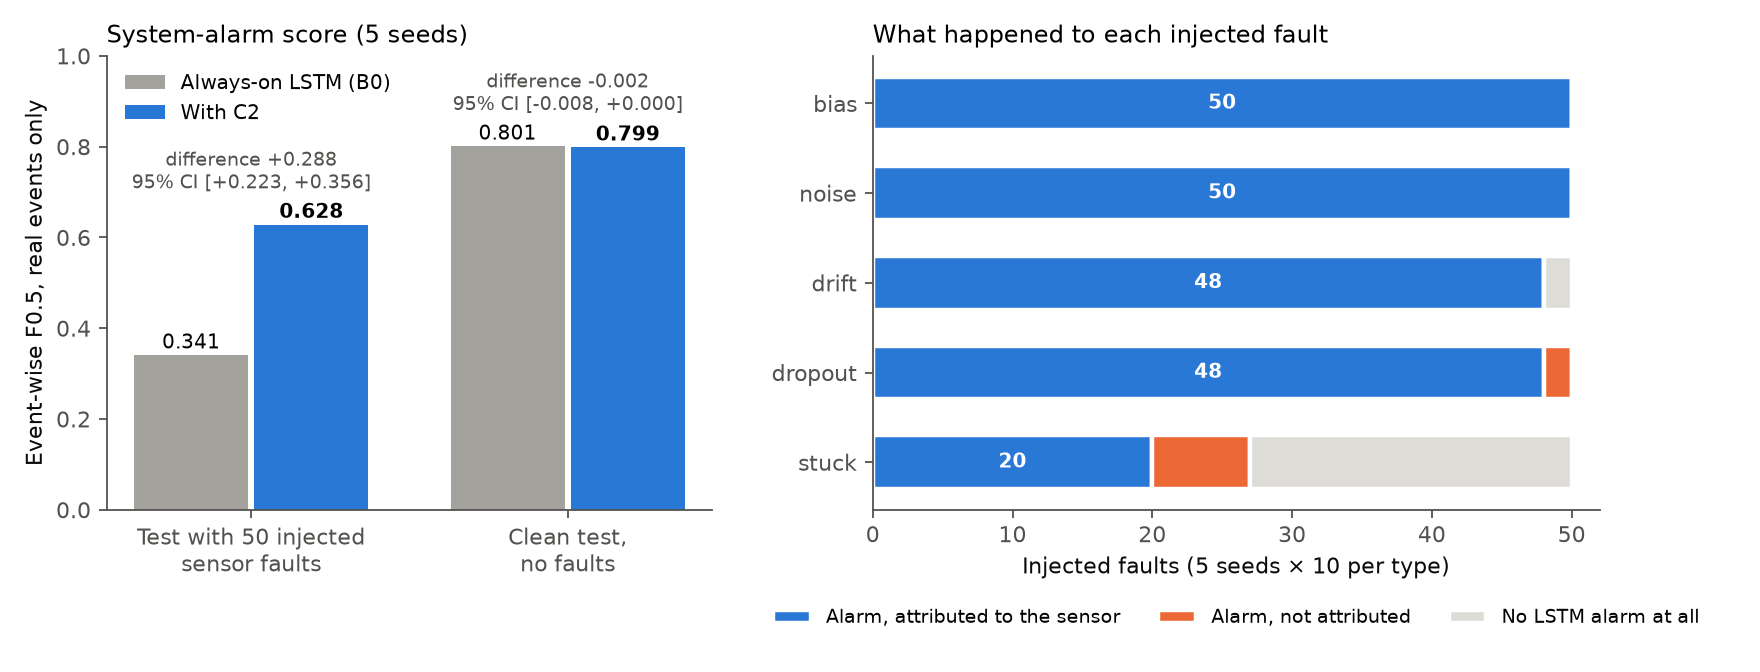
\includegraphics[width=0.88\textwidth]{figures/8_c2_sensor_reliability.png}
\caption{C2. Left: system-alarm F0.5 against real events, with and without C2. Right: outcome of each injected fault by type (test period, 5 seeds $\times$ 10 faults per type).}
\label{fig:c2}
\end{figure*}

\subsection{Calibrated error floor (H1)}
The Pruned floor of 0.007 was hand-picked. We choose a floor from \{0, 0.003, 0.005, 0.007, 0.01, 0.015, 0.02, 0.03\} by mean development F0.5. H1 states that the chosen floor improves test F0.5.

\subsection{C1: adaptive computation (H2)}
A cheap tier scores every sample with three signals:
\begin{itemize}
\item \emph{confidence:} the residual of a 12-lag linear forecaster;
\item \emph{novelty:} the Mahalanobis distance of 1-hour rolling means and spreads;
\item \emph{impact:} the number of channels deviating at once.
\end{itemize}
Each signal is converted to a rank against nominal training data. A trigger above threshold $\tau$ opens an LSTM burst: 2,400 warm-up samples, then 2,100 samples of look-back before the trigger and 2,100 after it. The warm-up rebuilds the error history the threshold needs. Every sample in a burst counts as LSTM work.

The LSTM is stateless given its input window, so routing can be simulated exactly from the full forecasts. The protocol picks the smallest LSTM share whose development F0.5 is within 0.01 of the always-on LSTM. H2 claims non-inferiority.

\begin{table*}[t]
\caption{All confirmatory test-set results (5 seeds, paired monthly-block bootstrap)}\label{tab:summary}
\centering
\begin{tabular}{lllll}
\toprule
Hypothesis & Comparison & Result & 95\% CI & Verdict \\
\midrule
H1 floor & floor 0.005 vs 0.007 & F0.5 0.818 vs 0.801 & $[-0.009, +0.055]$ & not confirmed \\
H2 / C1 & adaptive vs always-on LSTM & F0.5 0.801 vs 0.801; LSTM share 6.4\% & $[0.000, 0.000]$ & \textbf{non-inferior} \\
H3a / C2 & injected faults, with vs without C2 & F0.5 0.628 vs 0.341 & $[+0.223, +0.356]$ & \textbf{improvement} \\
H3b / C2 & clean data, with vs without C2 & F0.5 0.799 vs 0.801 & $[-0.008, 0.000]$ & \textbf{non-inferior} \\
H4 / C3 & learned graph G2 vs time-only G1 & pairwise F1 0.406 vs 0.978 & $[-0.576, -0.179]$ & worse \\
H5 / C4 & learned policy P2 vs P0 and P1 & best at 12 of 36 grid points & --- & not supported \\
H6 rare & telecommand gates vs baseline & F0.5 0.835 vs 0.801 & $[-0.017, +0.096]$ & not confirmed \\
\bottomrule
\end{tabular}
\end{table*}

\subsection{C2: sensor reliability (H3a, H3b)}
ESA-ADB has no sensor-fault labels, so we inject 50 single-channel faults per period: 10 each of stuck, drift, bias, noise and dropout. The faults last 2--24\,h, are sized in units of the channel's training standard deviation, and never overlap labelled events. The seeds are fixed in advance.

For each alarm, C2 computes seven features:
\begin{itemize}
\item the number of channels involved and the share of the top channel;
\item how much the top channel disagrees with a linear prediction from its five peers, relative to the other channels;
\item stuck, noise and out-of-range indicators.
\end{itemize}
A logistic model gives P(sensor fault). Alarms above a threshold become maintenance tickets and leave the system-alarm stream. The model and threshold are fitted on development alarms only: the threshold maximises sensor-fault F1 with at most 5\% of real-event alarms suppressed. H3a claims improvement on the injected test set. H3b claims non-inferiority on the clean test set.

\subsection{C3: incident correlation (H4)}
On all 76 channels, a univariate autoregressive detector per channel raises alerts above its 99.99th training percentile. G0 treats every alert as an incident. G1 merges alerts within $W$ samples. G2, the proposed method, merges them only if their channels are linked in a graph learned from the correlation of training residual activity at threshold $\rho$. $W$ and $\rho$ are tuned on development data. H4 states that G2 beats G1 in pairwise grouping F1 against ESA event IDs.

\subsection{C4: cost-aware response replay (H5)}
Each alarm on the faulty test period is paged, ticketed or ignored. Costs are defined over its true class (anomaly, rare event, sensor fault or false alarm) and a declared grid of 36 points. The grid varies the cost of ignoring an anomaly, delaying it, a false page and a missed sensor fault.

We compare four policies:
\begin{itemize}
\item \emph{P0:} page every alarm.
\item \emph{P1:} the C2 rule: ticket if C2 says sensor fault, otherwise page.
\item \emph{P2:} a multinomial class model trained on development alarms, choosing the action with the lowest expected cost.
\item \emph{Oracle:} knows the true class.
\end{itemize}
H5 requires P2 to have lower regret than P0 and P1 at $\geq$80\% of grid points. This is a replay of the alert policy, not of the spacecraft.

\subsection{Telecommand-gated rare-event path (H6)}
In the development period, high-priority telecommands (priority $\geq 2$) preceded 9 of 16 rare events within 30 minutes and none of 17 anomalies. The 30 minutes after them cover only 0.1\% of the time.

After each such command a gate opens for $W$. Inside the gate, the LSTM alarms at a lower floor $f_r$; outside gates the baseline is unchanged. We grid $p \in \{2,3\}$, $W \in \{0.5, 1, 3\}$\,h and $f_r \in \{0, 0.003, 0.005\}$ on development data. H6 states that F0.5 improves on the baseline. Telecommands are a model input that operators know in real time; they are not labels.

\section{Results}
\begin{figure*}[t]
\centering
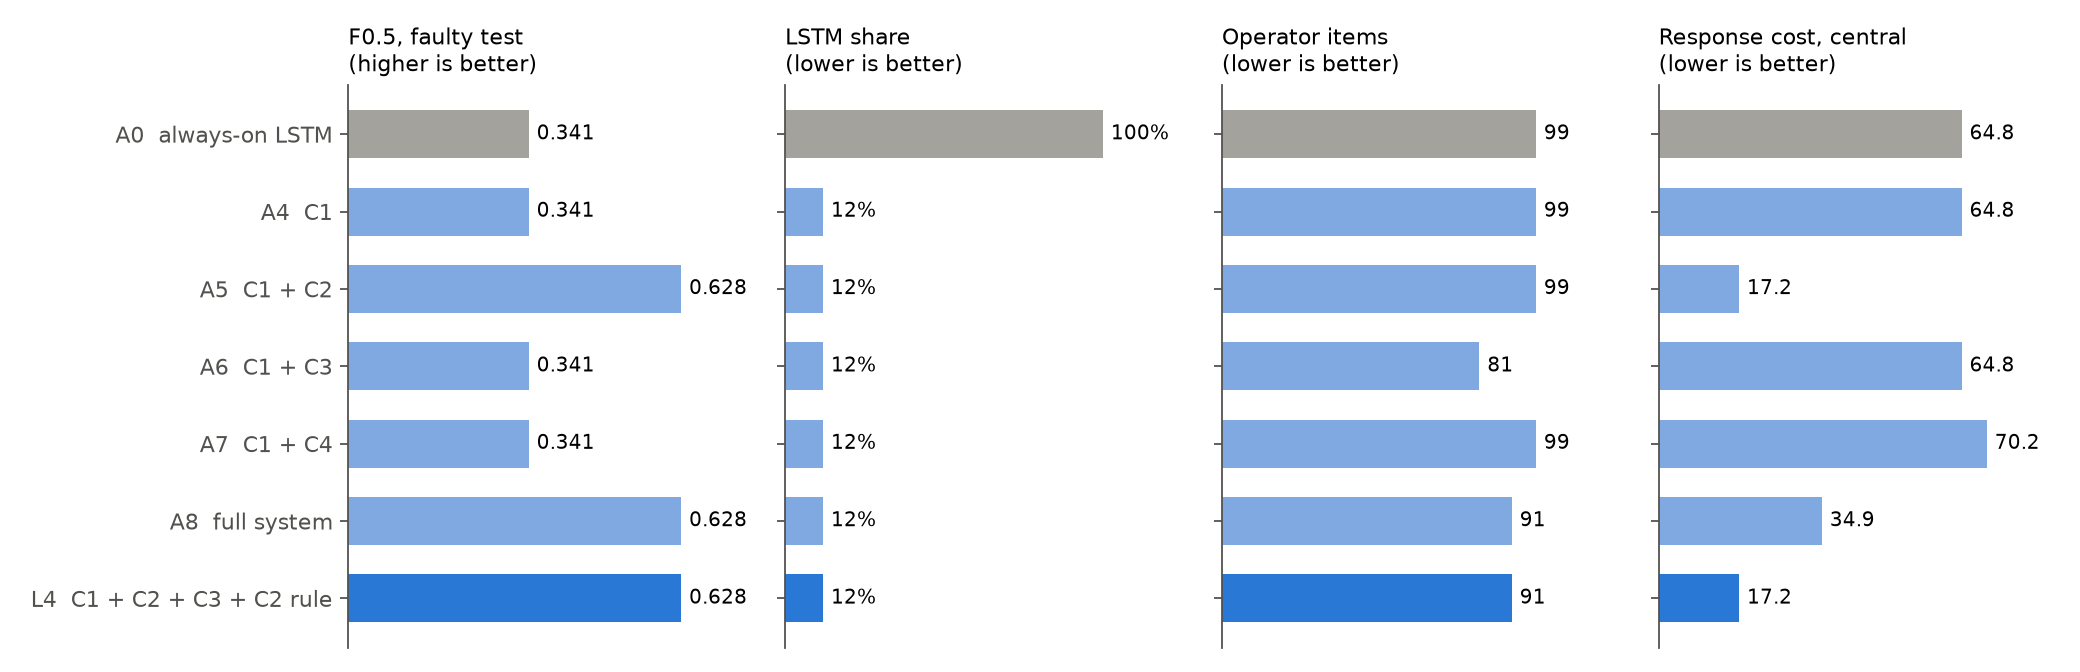
\includegraphics[width=0.88\textwidth]{figures/11_c5_ablation.png}
\caption{C5 ablation on the test period with injected sensor faults (5 seeds). A0: always-on LSTM; A4: C1; A5--A7: C1 plus one of C2--C4; A8: full system; L4: A8 with the C2 rule in place of the learned C4 policy.}
\label{fig:c5}
\end{figure*}

\begin{figure*}[t]
\centering
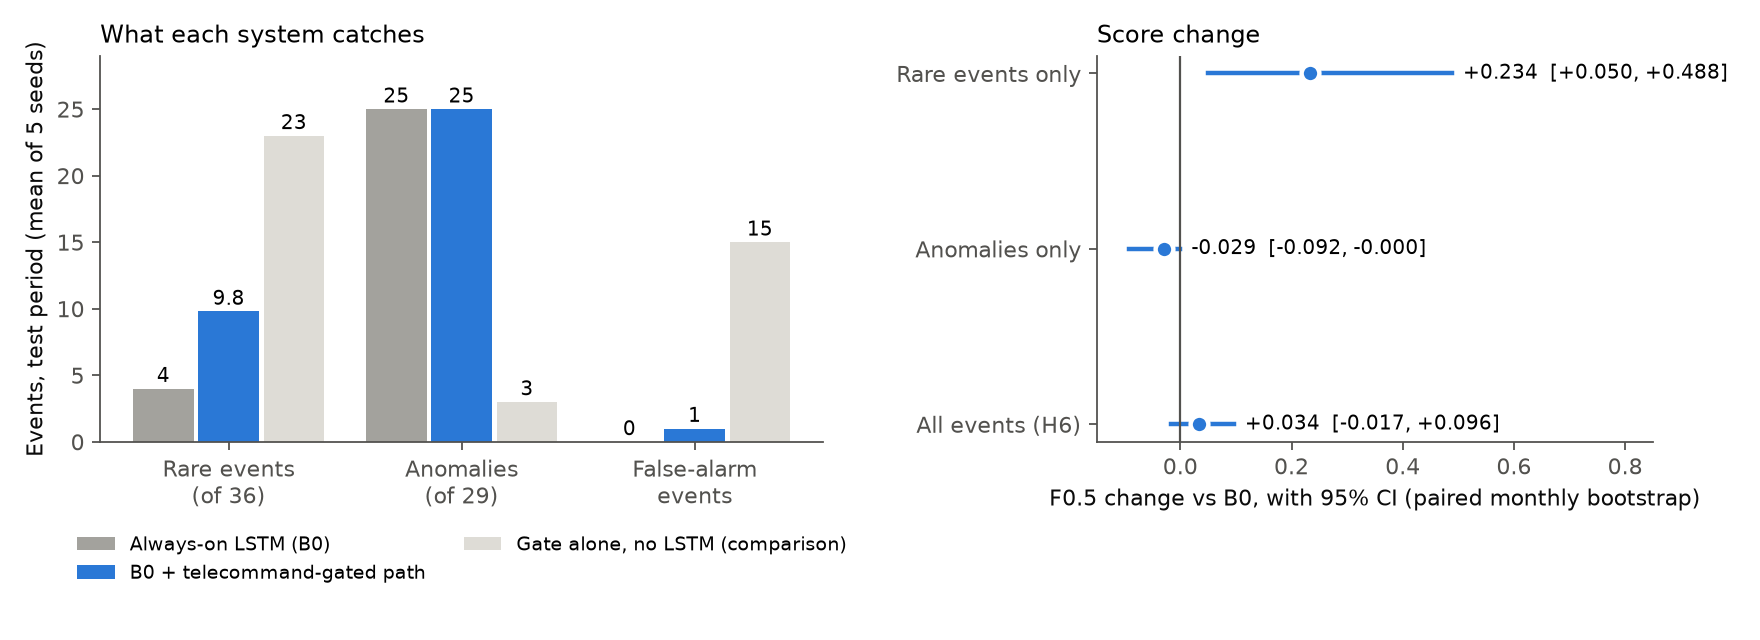
\includegraphics[width=0.88\textwidth]{figures/12_rare_events.png}
\caption{Telecommand-gated rare-event path. Left: events caught and false alarms (test period, mean of 5 seeds). Right: F0.5 change against the baseline with 95\% intervals.}
\label{fig:rare}
\end{figure*}

Table~\ref{tab:summary} summarises every test-set run.

\begin{table}[t]
\caption{C3 on all 76 channels, test period}\label{tab:c3}
\centering
\begin{tabular}{lccc}
\toprule
Grouping & Pairwise F1 & Incidents/event & Mixed incidents \\
\midrule
G0 none & 0.000 & 30.24 & 0 \\
G1 time only & \textbf{0.978} & \textbf{1.48} & 4 \\
G2 learned graph & 0.406 & 7.41 & 1 \\
G2 with subsystems & 0.893 & 1.64 & 1 \\
\bottomrule
\end{tabular}
\end{table}

\subsection{Calibrated floor}
Floor 0.005 was best on all five seeds in development (0.816 vs 0.776). On the test set it finds 2--3 more rare events and scores 0.818 against 0.801, but the interval includes zero. With 65 test events, a gain of about 0.02 F0.5 is within resampling noise.

\subsection{C1: adaptive computation}
At $\tau=0.999$ the router held the always-on development score at 12.3\% LSTM share (Fig.~\ref{fig:c1}). On the test set it catches exactly the same events with the same false alarms on every seed. The interval is $[0, 0]$, with the LSTM running on 6.4\% of the data (mean of 5 seeds).

We measured timing on seed~42, whose routed run has 52 bursts, in a single session. Inference takes 844\,s for the always-on LSTM and 29\,s for the routed LSTM plus 12\,s for screening, an end-to-end speed-up of 20.3$\times$. At the most aggressive thresholds the novelty and impact signals matter: at $\tau=0.9999$ they keep development F0.5 at 0.752 against 0.730 for confidence alone.

\subsection{C2: sensor reliability}
The development threshold of 0.498 gives a development sensor-fault F1 of 0.949 and suppresses 3 of 114 real-event alarms. On the faulty test period, every fault the LSTM notices becomes a false system alarm and F0.5 drops to 0.341. C2 restores it to 0.628, a gain of $+0.288$ (Fig.~\ref{fig:c2}). On clean data C2 removed one real-event alarm in one of five seeds (0.799 vs 0.801).

By fault type, bias, noise, drift and dropout faults are almost always alarmed and attributed (96--100\%). Stuck sensors are the weak spot: only 27 of 50 raise an LSTM alarm at all, because a frozen value can look nominal, and 20 of those 27 are attributed.

\subsection{C3: incident correlation}
The test period has 22,420 channel alerts, 1,996 of them on labelled events (Table~\ref{tab:c3}). Time-only grouping (G1, $W=720$) cuts operator load from 30.2 alerts per event to 1.48 incidents, with pairwise F1 0.978. The learned graph (G2, $W=2880$, $\rho=0.1$) never merges two events (precision 1.000) but splits most real incidents (recall 0.254). Training data contains too few incidents to learn reliable links, and the development period showed the same pattern (G2 0.801 vs G1 0.897). ESA's subsystem list, used as the graph instead, does far better than the learned one (F1 0.893, precision 1.000).

\subsection{C4: cost-aware response}
The faulty test period yields 170 anomaly, 20 rare-event, 287 sensor-fault and 17 false alarms (5 seeds pooled). At the central grid point, paging everything costs 64.8 per test period, the C2 rule 17.2 and the learned policy 34.9. P1 ranks first at 24 of 36 grid points and P2 at 12. P0 never ranks first, and P1 beats it at every point.

P2 wins mainly when delaying a real anomaly is cheap. It never wins when delay is expensive, because it judges some real anomalies ticket-worthy. The learned model therefore adds risk, not value: once a reliable sensor-fault label exists, a one-line rule is the better policy.

\subsection{C5: ablation}
Fig.~\ref{fig:c5} combines the components on the faulty test period:
\begin{itemize}
\item \emph{C2} is the only component that changes F0.5. Removing it loses the full $+0.288$.
\item \emph{C1} keeps every score at 11.9\% LSTM share (6.4\% on clean data). The cheap tier alone, without the LSTM, collapses to F0.5 0.106 with 4.6 times as many alarms.
\item \emph{Time grouping} cuts operator items from 98.8 to 81.0. In the full system it cuts them to 91.2, because sensor tickets and system alarms are grouped separately. No incident ever mixed a real event with an injected fault.
\item \emph{The learned C4 policy} raises the cost from 17.2 to 34.9 against the C2 rule.
\end{itemize}
The best combination is therefore C1 + C2 + time grouping + the C2 rule.

\subsection{Rare events}
The development grid chose priority $\geq 2$, $W=3$\,h and $f_r=0.003$, raising development F0.5 from 0.776 to 0.891. The gates cover 0.4\% of the test period.

On the test set (Fig.~\ref{fig:rare}) the path catches 9.8 of 36 rare events against 4, with no anomaly lost and one added false alarm. Rare-event F0.5 improves clearly: $+0.234$, 95\% CI $[+0.050, +0.488]$. The overall gain of $+0.034$ is not confirmed, however. The added false alarm counts against every category, so anomaly-only F0.5 falls by 0.029.

Gates alone, without the LSTM, find 23 rare events but raise 15 false alarms. Telecommands therefore carry most of the rare-event signal, and the LSTM confirmation inside the gate is the part to improve.

\section{Discussion}
\textbf{The decision layer matters most.} Five networks that make different predictions catch identical events, and every gain we confirmed acts after the forecaster: when it runs (C1) and which alarms are trusted (C2).

\textbf{Simple baselines are strong.} Time-only grouping beat the learned graph, and a one-line ticket rule beat the learned cost model. Both negative results were fixed in advance as hypotheses, which keeps such comparisons honest.

\textbf{Small event counts limit claims.} With 65 test events, effects of about 0.02--0.03 F0.5 (the calibrated floor, the rare-event path) cannot be confirmed even when they appear on every seed. Larger channel sets or further missions are needed to settle them.

\section{Limitations}
\begin{itemize}
\item \emph{Data:} the LSTM results cover one six-channel group of one mission.
\item \emph{Sensor faults:} the faults are injected by a simple generator also used for development, so C2's result is likely optimistic for real failures.
\item \emph{Response costs:} C4 depends on a declared cost grid, not measured costs.
\item \emph{Anonymised data:} channels and telecommands are anonymised, so learned dependencies are statistical, not physical.
\item \emph{Framework port:} our PyTorch port differs numerically from the original, which shows in the unpruned variant.
\item \emph{Timing:} timings come from a single laptop.
\end{itemize}

\section{Conclusion}
We reproduced Telemanom-ESA on ESA-ADB and tested six additions under a pre-registered protocol. Adaptive computation keeps detection unchanged while running the LSTM on 6.4\% of the data, 20.3$\times$ faster. A peer-consistency sensor-reliability layer nearly doubles F0.5 when sensors fail, without harming clean data. Learned incident graphs and learned response policies did not beat simpler alternatives. Telecommand gating more than doubled rare-event detections, but its overall gain is not confirmed. Code, protocol, test log and results are available in the project repository.

\bibliographystyle{IEEEtran}
\bibliography{refs}

\end{document}
